\iffalse
\documentclass[10pt,a4paper]{report}
%\usepackage[latin1]{inputenc}
\usepackage[utf8]{inputenc}
\usepackage{amsmath}
\usepackage{amsfonts}
\usepackage{amssymb}
\usepackage{graphicx}
\usepackage{multicol}
\usepackage{tabularx}
\usepackage{tikz}
\usetikzlibrary{arrows,shapes,automata,petri,positioning,calc}
\usepackage{hyperref}
\usepackage{tikz}
\usetikzlibrary{matrix,calc}
\usepackage[margin=0.5in]{geometry}
% ---- power functions -----% 
\newcommand{\myvec}[1]{\ensuremath{\begin{pmatrix}#1\end{pmatrix}}}
\let\vec\mathbf

\providecommand{\norm}[1]{\left\lVert#1\right\rVert}
\providecommand{\abs}[1]{\left\vert#1\right\vert}
\let\vec\mathbf

\newcommand{\mydet}[1]{\ensuremath{\begin{vmatrix}#1\end{vmatrix}}}
\providecommand{\brak}[1]{\ensuremath{\left(#1\right)}}
\providecommand{\lbrak}[1]{\ensuremath{\left(#1\right.}}
\providecommand{\rbrak}[1]{\ensuremath{\left.#1\right)}}
\providecommand{\sbrak}[1]{\ensuremath{{}\left[#1\right]}}
%-------end power functions----%
\newenvironment{Figure}
  {\par\medskip\noindent\minipage{\linewidth}}
  {\endminipage\par\medskip}
\begin{document}
%--------------------logo figure-------------------------%
\begin{figure*}[!tbp]
  \centering
  \begin{minipage}[b]{0.4\textwidth}
    
\includegraphics[scale = 0.05]{iitlogo.jpg}
  \end{minipage}
  \hfill
  \vspace{5mm}\begin{minipage}[b]{0.4\textwidth}
\raggedleft  
\includegraphics[scale = 0.10]{nrc.png}\

  \end{minipage}\vspace{0.2cm}
\end{figure*}
%--------------------name & rollno-----------------------
\raggedright \textbf{Name}:\hspace{1mm} Chirag Shah\hspace{3cm} \Large \textbf{Assignment-6}\hspace{2.5cm} % 
\normalsize \textbf{Roll No.} :\hspace{1mm} FWC22053\vspace{1cm}
\begin{multicols}{2}

%----------------problem statement--------------%
\raggedright \textbf{Problem Statement:}\vspace{2mm}
\raggedright \\ 
\fi
	Find the area of the circle $4x^2+4y^2=9$ which is interior to the parabola $x^2=4y$.\\
	\solution
	\begin{figure}[!h]
		\centering
 \includegraphics[width=\columnwidth]{chapters/12/8/2/1/figs/conic.jpg}
		\caption{}
		\label{fig:12/8/2/1}
  	\end{figure}
	\iffalse
\vspace{5mm}
%-----------------------------solution---------------------------
\raggedright \textbf{SOLUTION}:\vspace{2mm}\\

%---------given----------------%
\raggedright \textbf{Given}:\vspace{2mm}\\
Equation of circle is \\
\begin{align}
4x^2+4y^2=9
\end{align}
Equation of Parabola is \\ 
\begin{align}
x^2=4y 
\end{align}
From (2) we can say that Parabola is concave towards positive y axis.\\ \vspace{2mm}
From equation (1) radius of circle is,\\ 
\begin{align}
r= \frac{3}{2}
\end{align}

%-------------To find ------------------%
\textbf{To Find }\vspace{2mm}\\
To find the intersection points and area of shaded region shown in figure\vspace{2mm}  \\ 
%--------------steps----------------------%
\textbf{STEP-1}\vspace{2mm}\\
\fi
The given circle and parabola can be expressed as conics with parameters 
\begin{align}
	\vec{V}_1&=4\vec{I},
\vec{u_1}=\vec{0},
f_1=-9
\\
	\vec{V}_2&=\myvec{
1 & 0\\
0 & 0
},
\vec{u_2}= -\myvec{
0\\
2
},
f_2=0
\end{align} 
\iffalse
\textbf{STEP-2}\vspace{2mm}\\
\fi
The intersection of the given conics is obtained
as
\begin{align}
	\vec{x}^{\top}\brak{\vec{V}_1 + \mu\vec{V}_2}\vec{x}+2 \brak{\vec{u}_1+\mu \vec{u}_2}^{\top} \vec{x} 
	+ \brak{f_1+\mu f_2}= 0
    \end{align}
    \iffalse
    where
\begin{align}
	\vec{V}_1+\mu\vec{V}_2&= \myvec{
\mu+4 & 0\\
0 & 4
}
\\
	\vec{u}_1+\mu\vec{u}_2&= -\myvec{
0\\
2\mu
}
f_1+\mu f_2= -9
\end{align}
\fi
This conic represents a pair of straight lines if
\begin{align}
\mydet{\vec{V}_1 + \mu\vec{V}_2 & \vec{u}_1+\mu \vec{u}_2\\ \brak{\vec{u}_1+\mu \vec{u}_2}^{\top} & f_1 + \mu f_2} &= 0
\end{align}
\iffalse
And,\\
\begin{align}
\mydet{\vec{V}_1 + \mu\vec{V}_2} &= 0
\end{align}
Substituting equation (13),(14) and (15) in equation (16)\\ 
We get,\\ 
\fi
which can be expressed as
\begin{align}
\implies \mydet{\mu+4 & 0 & 0\\ 
0 & 4 & -2\mu \\
0 & -2\mu & -9
} &= 0
\end{align}
Solving the above equation we get, 
\begin{align}
\mu^3 + 4\mu^2 + 9\mu + 36=0
\end{align}
yielding
\begin{align}
    \mu = -4.
\end{align}
 Thus, the parameters for the pair of  straight lines can be expressed as 
 \begin{align}
	\vec{V} &= 
\vec{V}_1 + \mu\vec{V}_2
=\myvec{ 0 & 0 \\ 0 & 4},
\\
	\vec{u} &=
\vec{u}_1+\mu \vec{u}_2
	= \myvec{
0\\
8
    }
\\
	f&=-9,
	\\
	\implies \vec{D} &= \vec{V}, \vec{P} = \vec{I}
    \end{align}
    \iffalse
Thus, the desired pair of straight lines are \\ 
\begin{align} 
	\myvec{\sqrt{\abs{\lambda_1}} & \pm \sqrt{\abs{\lambda_2}}}\vec{P}^{\top}\brak{\vec{x}-\vec{c}} &= 0
\end{align}
\begin{align}
	\implies\myvec{0 & \pm 2}\vec{x}-\vec{c} &= 0
\end{align}
\begin{align}
	\text{or, }\vec{x} =\vec{c} + \kappa \myvec{\pm 2 \\ 0}
\end{align} 
\iffalse
The points of intersection of the line is given by  
\begin{align}
L: \quad \vec{x} = \vec{q} + \kappa \vec{m} \quad \kappa \in \mathbb{R}
\end{align}
with the conic section, \\ 
\begin{align}
	\vec{x}^{\top}\vec{V}\vec{x} + 2\vec{u}^{\top} \vec{x} + f = 0
\end{align}
are given by \\
\begin{align}
\vec{x}_i = \vec{q} + \kappa_i \vec{m}
\end{align}
where, \\
{\tiny
\begin{multline}
\kappa_i = \frac{1}
{
\vec{m}^T\vec{V}\vec{m}
}
\lbrak{-\vec{m}^T\brak{\vec{V}\vec{q}+\vec{u}}}
\\
\pm
\rbrak{\sqrt{
\sbrak{
\vec{m}^T\brak{\vec{V}\vec{q}+\vec{u}}
}^2
-
\brak
{
\vec{q}^T\vec{V}\vec{q} + 2\vec{u}^T\vec{q} +f
}
\brak{\vec{m}^T\vec{V}\vec{m}}
}
}
\end{multline}
}
\fi
On substituting
\begin{align}
\vec{q} &= \myvec{
0\\
0.5
} 
\end{align}
\begin{align}
\vec{m} = \myvec{2 \\ 0}
\end{align}
With the given Parabola,\\ 
\begin{align}
	\vec{V} &= \myvec{
1 & 0\\
0 & 0
    }
\end{align}
\begin{align}
	\vec{u} = -\myvec{2 \\0}
 \end{align}
 \begin{align}
  f = 0
 \end{align}
The value of $\kappa$ ,\\
\begin{align}
    \kappa = \sqrt{2},-\sqrt{2}
\end{align}
The points of intersection with Parabola along circle are \\
\begin{align}
    \vec{A}=\myvec{
\sqrt{2}\\
0.5
    }
\end{align}
\begin{align}
    \vec{B}=\myvec{
-\sqrt{2}\\
0.5
    }
\end{align}
\textbf{Result}
\begin{center}
 \includegraphics[width=0.5\textwidth]{conic.jpg}  
 \end{center}
 From the figure,\\ 
Total area of portion is given by, \\ 
\begin{align}
 A=  \int_{-\sqrt{2}}^{\sqrt{2}} g(x)-f(x) \,dx 
\end{align}
Where g(x) is area of circle and f(x) is the area of parabola around the points\\ 
\begin{align}
A= \int_{-\sqrt{2}}^{\sqrt{2}} \frac{\sqrt{9-4x^2}}{2}-\frac{x^2}{4} \,dx 
\end{align}
Area A is,\\ 
\begin{align}
    A= 3.0053609 \,m^2
\end{align}
 \vspace{2mm} \textbf{Construction}
\begin{center}
\setlength{\arrayrulewidth}{0.5mm}
\setlength{\tabcolsep}{6pt}
\renewcommand{\arraystretch}{1.5}
    \begin{tabular}{|l|c|}
    \hline 
    \textbf{Points} & \textbf{coordinates} \\ \hline
   $\vec{A}$ & $\myvec{
   \sqrt{2}\\
   0.5
   } $ \\\hline
   $\vec{B}$ & $\myvec{
   -\sqrt{2}\\
   0.5
   } $ \\\hline
      \end{tabular}
  \end{center}

\raggedright  Download the code \\
Github link: \href{https://github.com/chiragshah1244/FWC/blob/main/assignments/assignment_6/code_conic/conic.py}{Assignment-6}.
  \end{multicols}
\end{document}
\fi
